\documentclass[a4paper,14pt]{extarticle}

\usepackage[utf8x]{inputenc}
\usepackage[T1,T2A]{fontenc}
\usepackage[russian]{babel}
\usepackage{hyperref}
\usepackage{indentfirst}
\usepackage{here}
\usepackage{array}
\usepackage[table]{xcolor}
\usepackage{datetime}
\usepackage{multirow}
\usepackage{hhline}
\usepackage{mathtools,cancel}
\usepackage{forest}
\usepackage{graphicx}
\usepackage{caption}
\usepackage{subcaption}
\usepackage{chngcntr}
\usepackage{amsmath}
\usepackage{amssymb}
\usepackage{pgfplots}
\usepackage{pgfplotstable}
\usepackage[left=2cm,right=2cm,top=2cm,bottom=2cm,bindingoffset=0cm]{geometry}
\usepackage{multicol}
\usepackage{askmaps}
\usepackage{tikz}

\newcommand*\circled[1]{\tikz[baseline=(char.base)]{
            \node[shape=circle,draw,inner sep=2pt] (char) {#1};}}

\DeclareMathOperator*{\argmin}{argmin}

\renewcommand{\not}[1]{\mkern 1.5mu\overline{\mkern-1.5mu#1\mkern-1.5mu}\mkern 1.5mu}
\renewcommand{\le}{\ensuremath{\leqslant}}
\renewcommand{\leq}{\ensuremath{\leqslant}}
\renewcommand{\ge}{\ensuremath{\geqslant}}
\renewcommand{\geq}{\ensuremath{\geqslant}}
\renewcommand{\epsilon}{\ensuremath{\varepsilon}}
\renewcommand{\phi}{\ensuremath{\varphi}}

\counterwithin{figure}{section}
\counterwithin{equation}{section}
\counterwithin{table}{section}
\newcommand{\sign}[1][5cm]{\makebox[#1]{\hrulefill}} % Поля подписи и даты
\graphicspath{{pics/}} % Путь до папки с картинками
\captionsetup{justification=centering,margin=1cm}
\def\arraystretch{1.3}

\begin{document}

\begin{titlepage}
\begin{center}
	Санкт-Петербургский политехнический университет Петра Великого\\[0.3cm]
	Институт компьютерных наук и технологий \\[0.3cm]
	Кафедра компьютерных систем и программных технологий\\[4cm]
	
	\textbf{Расчётное задание №6}\\[2mm]
	\textbf{Дисциплина:} Системный анализ и принятие решений\\[2mm]
	\textbf{Тема:} Дискретное программирование. Задача коммивояжёра\\[2mm]
	Вариант 39\\[6.5cm]
\end{center}

\begin{flushleft}
	\hspace*{5mm} Выполнил студент гр. 33501/4  \hspace*{3cm}\sign[3cm]\hspace*{2mm} А.Ю. Ламтев\\
	\hspace*{10.85cm} (подпись)\\[2.5mm]
	\hspace*{5mm} Преподаватель \hspace*{6.45cm}\sign[3cm]\hspace*{2mm} С.С. Сабонис\\
	\hspace*{10.85cm} (подпись)\\[2.5mm]
	\hspace*{11.1cm} <<\underline{\the\day}>> \underline{\hspace{5mm}ноября\hspace{5mm}} \the\year\hspace{1mm} г.
\end{flushleft}

\vfill

\begin{center}
	Санкт-Петербург\\
	\the\year
\end{center}
\end{titlepage}
\addtocounter{page}{1}

\section{Задание}

\begin{displaymath}
\begin{cases}
	max \left( x_1 + 2 \cdot x_2 \right)
	\\
	x_1 + x_2 \leq 5.7
	\\
	x_1 - x_2 \leq 1.6
	\\
	x_1 \geq 0
	\\
	x_2 \geq 0
\end{cases}
\end{displaymath}

\begin{enumerate}

	\item Привести задачу к канонической форме.
	
	\item Решить задачу геометрическим методом.
	
	\item Обозначить все опорные точки (в том числе недопустимые) и записать соответствующие им наборы базисных переменных, рассчитать значение целевой функции в каждой опорной точке (решить задачу методом полного перебора опорных точек).
	
	\item Решить задачу симплекс-методом в матричной форме.	
	
	\item Решить задачу симплекс-методом в табличной форме.

	\item Ввести дополнительное ограничение, отсекающее оптимальную точку. Решить новую задачу двойственным симплекс-методом в табличной форме, в качестве начального базиса новой задачи использовать оптимальный базис исходной задачи.
	
	\item Сформулировать задачу, двойственную по отношению к исходной.

\end{enumerate}

\section{Решение}

\begin{enumerate}
	
\item Приведём задачу к канонической форме:

\begin{equation}
\begin{cases}
	max \left( x_1 + 2 \cdot x_2 \right)
	\\
	x_3 = 5.7 - x_1 - x_2
	\\
	x_4 = 1.6 - x_1 + x_2
	\\
	x_1 \geq 0
	\\
	x_2 \geq 0
	\\
	x_3 \geq 0	
	\\
	x_4 \geq 0
\end{cases}
\end{equation}	

\item Решим задачу геометрическим методом.

\begin{figure}[H]
\begin{center}
	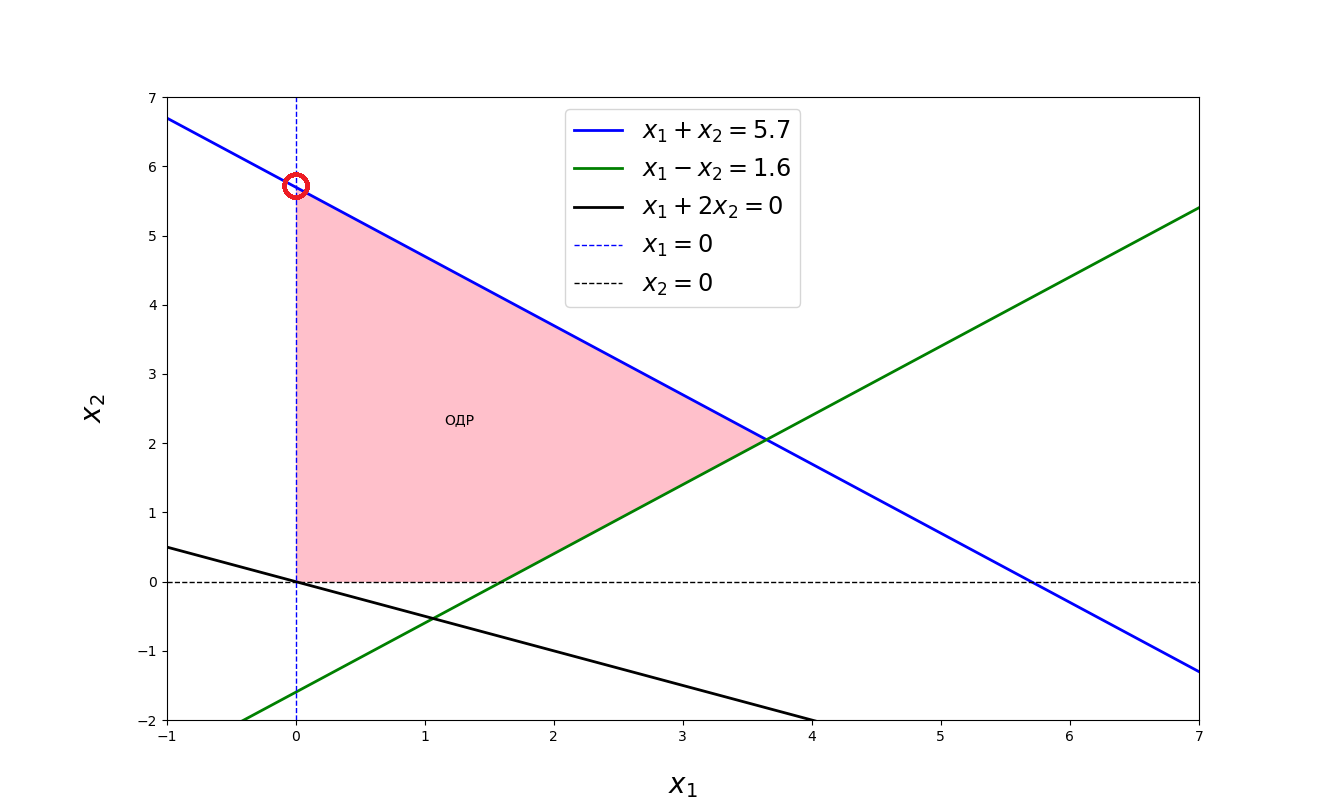
\includegraphics[width=1\textwidth]{geometric-solution}
	\caption{Геометрическое решение}
	\label{pic:graphic-solution}
\end{center}
\end{figure}

На рис. \ref{pic:graphic-solution} представлено геометрическое решение.

\item Решим задачу методом полного перебора опорных точек.\\
\noindent Для этого обозначим все опорные точки, запишем соответствующие им наборы базисных переменных и рассчитаем значение целевой функции в каждой опорной точке.

\end{enumerate}

\end{document}